\section{Gario Miordano}\label{gario-miordano}

Tags: PC Alias: Spaccazzucca Creatore: Davide Giocatore: Davide
Ispirazione: Mario Giordano Luogo: Azura Razza: Elfo Classe: Paladino
Livello: 5

\section{Gario Miordano}\label{gario-miordano-1}

\begin{center}\rule{0.5\linewidth}{0.5pt}\end{center}

\begin{figure}
\centering
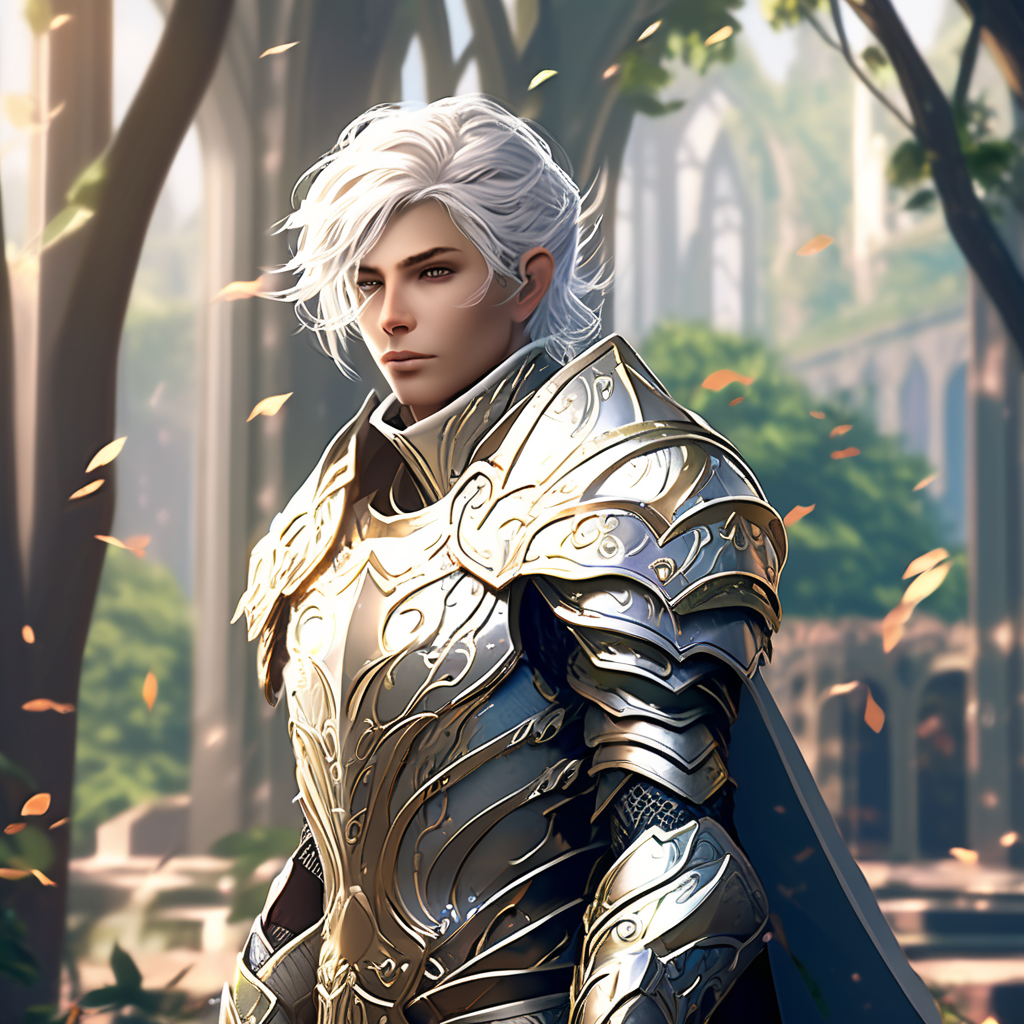
\includegraphics{depict-an-elf-paladin-he-is-a-young-adult-with-short-white-hairs-wearing-full-plate-armour.png}
\caption{depict-an-elf-paladin-he-is-a-young-adult-with-short-white-hairs-wearing-full-plate-armour.png}
\end{figure}

Informazioni Generali

Età: 623

Data di nascita:

Luogo di nascita: Fredo Flu

Razza: Elfo

Classe: Paladino

Alleati:

Nemesi: Le Zucche

Alias:

Professione:

\begin{center}\rule{0.5\linewidth}{0.5pt}\end{center}

\subsection{1. Descrizione Generale}\label{descrizione-generale}

\begin{center}\rule{0.5\linewidth}{0.5pt}\end{center}

\begin{figure}
\centering
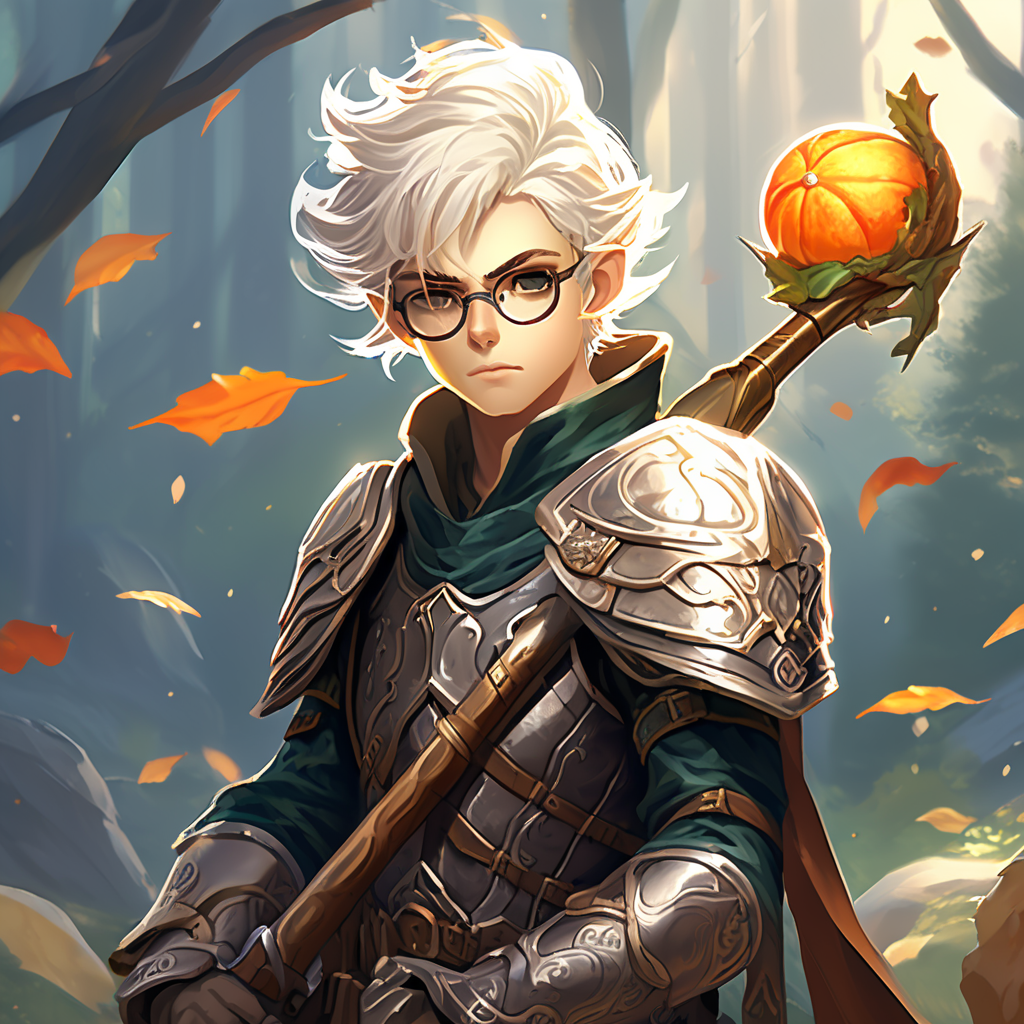
\includegraphics{depict-an-elf-paladin-he-is-a-young-adult-with-short-white-hairs-wearing-full-plate-armour-and-spe-923031639.png}
\caption{depict-an-elf-paladin-he-is-a-young-adult-with-short-white-hairs-wearing-full-plate-armour-and-spe-923031639.png}
\end{figure}

Gario è un elfo paladino di Fredo Flu, con una personalità complessa.
Sebbene animato da un senso di giustizia, è bigotto, xenofobo e
ipocrita, credendo di agire per il bene supremo. Dietro la durezza, ha
un cuore compassionevole, ma le sue azioni spesso suscitano polemiche.

\begin{quote}
``Io le feste di autunno non le voglio festeggiare'' - Gario Miordano
\end{quote}

\subsection{2. Biografia}\label{biografia}

\begin{center}\rule{0.5\linewidth}{0.5pt}\end{center}

\subsubsection{\texorpdfstring{\textbf{2.1 Origini Nobili e Caduta di
Fredo
Flu}}{2.1 Origini Nobili e Caduta di Fredo Flu}}\label{origini-nobili-e-caduta-di-fredo-flu}

Gario Miordano è nato all'interno di una delle più illustri famiglie
elfiche di Fredo Flu, un tempo una delle città più fiorenti e prosperose
del regno elfico. Cresciuto tra l'agio e il lusso, Gario ha goduto di
una vita privilegiata fin dalla sua infanzia, circondato dall'amore e
dall'attenzione della sua famiglia. Tuttavia, la sua vita idilliaca è
stata sconvolta quando una terribile maledizione ha colpito la famiglia
reale di Fredo Flu, causando la sua disfatta e il declino della città.

\subsubsection{\texorpdfstring{\textbf{2.2 Fuga a Pandosia e
Coinvolgimento
Politico}}{2.2 Fuga a Pandosia e Coinvolgimento Politico}}\label{fuga-a-pandosia-e-coinvolgimento-politico}

Costretto a fuggire insieme alla sua famiglia per sfuggire al destino
che stava per abbattersi su di loro, Gario ha trovato rifugio nella
città di Pandosia, dove è stato accolto da uno dei signori locali.
Durante la sua adolescenza a Pandosia, Gario si è trovato immerso in un
mondo di politica e intrighi, affascinato dalla complessità del potere e
delle relazioni sociali. La sua ambizione lo ha spinto ad avvicinarsi
sempre di più alla scena politica della città, fino a quando non ha
deciso di candidarsi a sindaco.

\subsubsection{\texorpdfstring{\textbf{2.3 La Sconfitta e la Profonda
Depressione}}{2.3 La Sconfitta e la Profonda Depressione}}\label{la-sconfitta-e-la-profonda-depressione}

Tuttavia, la sua candidatura è stata un fallimento e Gario è stato
sopraffatto da una profonda depressione, incapace di accettare la
sconfitta e il fallimento dei suoi sogni. In preda alla disperazione, ha
abbandonato Pandosia e ha iniziato un lungo viaggio attraverso terre
sconosciute, vagando senza meta per circa cinquant'anni.

\subsubsection{\texorpdfstring{\textbf{2.4 Il Giuramento e la Rinascita
Come
Paladino}}{2.4 Il Giuramento e la Rinascita Come Paladino}}\label{il-giuramento-e-la-rinascita-come-paladino}

Sulla soglia dei cinquecento anni di età, Gario è giunto in un antico
monastero nascosto tra le montagne, dove ha trovato rifugio e
consolazione. Qui, immerso nella solitudine e nella contemplazione, ha
trovato la fede e ha deciso di prestare giuramento come paladino,
dedicando la sua vita al servizio degli altri e alla difesa dei deboli e
degli oppressi.

\subsubsection{\texorpdfstring{\textbf{2.5 La Leggenda dello
Spaccazzucca}}{2.5 La Leggenda dello Spaccazzucca}}\label{la-leggenda-dello-spaccazzucca}

Durante i suoi vagabondaggi, Gario si trovò ad affrontare una minaccia
inaspettata: una banda di briganti malvagi che aveva preso d'assalto un
villaggio agricolo. Questi briganti, noti per la loro crudeltà, avevano
preso il controllo del villaggio e avevano iniziato a saccheggiare le
colture di zucche, essenziali per la sopravvivenza della comunità.
Gario, mosso dalla compassione per gli abitanti del villaggio e
determinato a porre fine alla tirannia dei briganti, affrontò i
malviventi con coraggio e astuzia.

Durante la battaglia che ne seguì, Gario afferrò una grande mazza di
legno e la usò con grande maestria contro i suoi avversari. Con ogni
colpo, le zucche che i briganti avevano rubato dal villaggio si
frantumavano sotto la forza travolgente della mazza di Gario. Il suono
sordo degli schianti delle zucche riempiva l'aria mentre Gario
combatteva con ferocia e determinazione. Alla fine, grazie alla sua
abilità nel combattimento e alla sua astuzia, Gario riuscì a sconfiggere
i briganti e a restituire la pace e la sicurezza al villaggio. Da quel
giorno in poi, Gario fu conosciuto come ``Lo Spaccazzucca'', in onore
della sua impresa eroica che aveva visto le zucche rotolare sotto la sua
mazza come se fossero state fatte di vetro.

\subsection{3. Carriera}\label{carriera}

\begin{center}\rule{0.5\linewidth}{0.5pt}\end{center}

\subsubsection{3.1 Carriera Politica}\label{carriera-politica}

Durante il periodo trascorso a Pandosia, Gario Miordano si immerse
attivamente nella politica locale, attratto dalla complessità dei giochi
di potere e dalle dinamiche sociali della città. Pur non essendo ancora
direttamente coinvolto nella politica ufficiale, Gario partecipò
attivamente alle discussioni comunitarie e alle riunioni pubbliche,
esprimendo le sue opinioni su questioni di interesse cittadino e
sostenendo cause che riteneva giuste e importanti. La sua voce risuonava
con autorità e rispetto tra i suoi concittadini, che apprezzavano la sua
sincerità e la sua dedizione alla causa del bene comune. Questa
esperienza lo ha preparato per la sua futura carriera politica,
fornendogli le basi necessarie per affrontare le sfide e le
responsabilità che avrebbe incontrato nel corso della sua vita pubblica.

\subsubsection{\texorpdfstring{\textbf{3.2 Carriera Come
Paladino}}{3.2 Carriera Come Paladino}}\label{carriera-come-paladino}

Dopo aver giurato fedeltà al monastero e aver abbracciato la vita da
paladino, Gario Miordano ha dedicato ogni istante della sua esistenza
alla difesa dei deboli e alla lotta contro le forze del male. Grazie
alla sua abilità nel combattimento e alla sua fede incrollabile, ha
affrontato numerosi nemici, da orde di creature oscure a potenti maghi
oscuri, dimostrando sempre una straordinaria determinazione e coraggio.
La sua reputazione di paladino valoroso e intraprendente si è diffusa
rapidamente, guadagnandogli il rispetto e l'ammirazione di coloro che
hanno avuto la fortuna di combattere al suo fianco. Attraverso le sue
imprese eroiche e il suo impegno costante per la giustizia e la
rettitudine, Gario continua a incarnare gli ideali dei Protettori,
servendo come esempio luminoso di sacrificio e dedizione per tutti
coloro che lo incontrano.

\subsection{4. Personalità}\label{personalituxe0}

\begin{center}\rule{0.5\linewidth}{0.5pt}\end{center}

Gario Miordano è caratterizzato da un atteggiamento bigotto, xenofobo e
ipocrita, sebbene sia convinto di agire per il bene supremo. La sua
rigida interpretazione delle sue credenze e la sua mancanza di
tolleranza nei confronti di chi è diverso da lui lo portano spesso a
manifestare pregiudizi e discriminazioni verso altre razze e culture.
Pur professando di difendere gli ideali di giustizia e moralità, Gario
mostra spesso un duplice standard nel trattare gli altri, giudicando
severamente i peccati altrui mentre giustifica i suoi stessi
comportamenti discutibili. La sua ipocrisia emerge quando, nonostante le
sue azioni discriminatorie, crede fermamente di essere dalla parte della
rettitudine e della verità. In certi momenti, Gario può dimostrare
generosità e compassione, ma spesso queste qualità sono riservate solo a
coloro che condividono le sue stesse convinzioni, mentre gli altri
vengono trattati con disprezzo e ostilità. In definitiva, la personalità
di Gario Miordano è contraddistinta da una complessa intersezione di
bigottismo, xenofobia e ipocrisia, che lo rende un individuo controverso
e difficile da comprendere.

\subsection{A. Coinvolgimenti in Eventi
Recenti}\label{a.-coinvolgimenti-in-eventi-recenti}

\begin{center}\rule{0.5\linewidth}{0.5pt}\end{center}

\href{Untitled\%20Database\%20d1df3a4c45d8458898cd664d89bf227a.csv}{Untitled
Database}

\subsection{B. Aggiornamenti}\label{b.-aggiornamenti}

\begin{center}\rule{0.5\linewidth}{0.5pt}\end{center}

\href{Untitled\%20878d7951acff43338f7728378c4730bf.csv}{}
